\chapter{Introducción}
\label{cap:introduccion}
Hoy en día debido a la gran cantidad de usuarios en los videojuegos en diferentes regiones, surge la necesidad de adaptar el videojuego a otras regiones o países diferentes al origen, para ello existe una serie de pasos o estrategias que se puede seguir, en mi caso diseñare una herramienta que ayude a este proceso.
\section{Motivación}
Con el paso de los años, los videojuegos se han convertido en una de las industrias de entretenimiento más grandes del mundo. Según un informe de \cite{NZIngreso2024}, en 2024, el mercado global de los videojuegos ha alcanzado un valor estimado de 187.7 miles de millones de ingreso como se muestra en la figura \ref{fig:NewZooRevenues}. En el mismo informe aparece el crecimiento jugadores (Figura \ref{fig:NewzooPlayers}), desde 3.14 billones en 2022 a 3.422 billones 2024 y su predicción en 2027 es de 3.759 billones.
\begin{figure}[H]
	\centering
	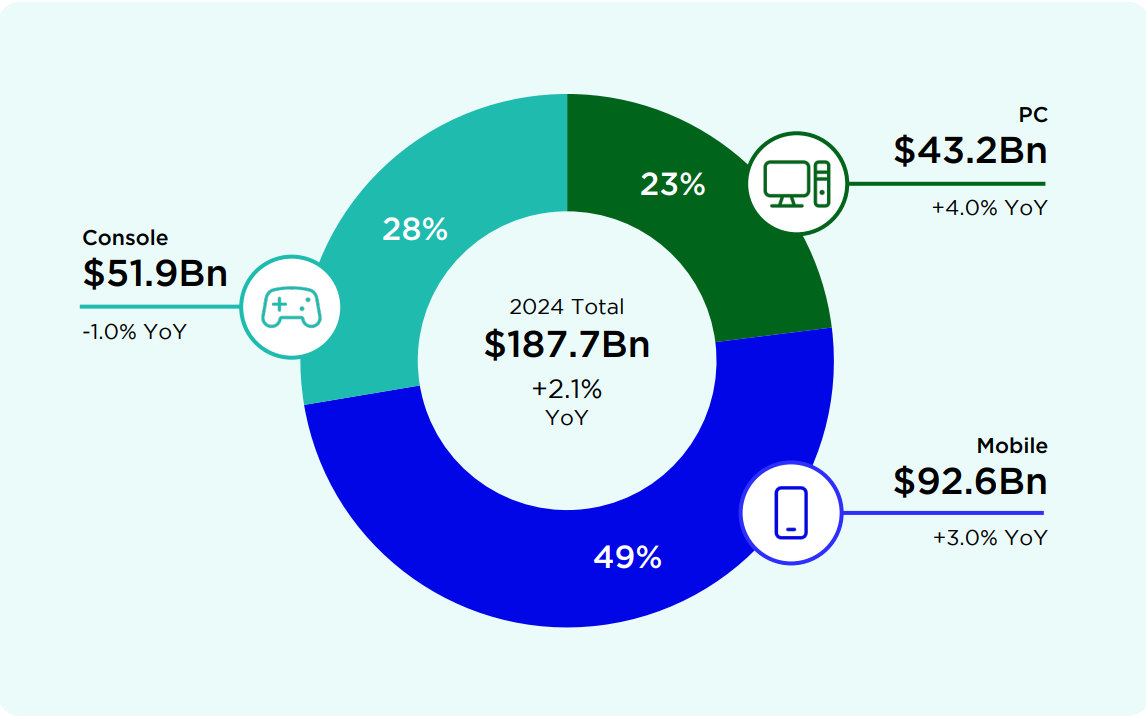
\includegraphics[width = 0.5\textwidth]{Imagenes/Newzoo_2024_Revenues.png}
	\caption{Ingreso estimado en la industria de videojuegos 2024.Newzoo}
	\label{fig:NewZooRevenues}
\end{figure}

\begin{figure}[H]
	\centering
	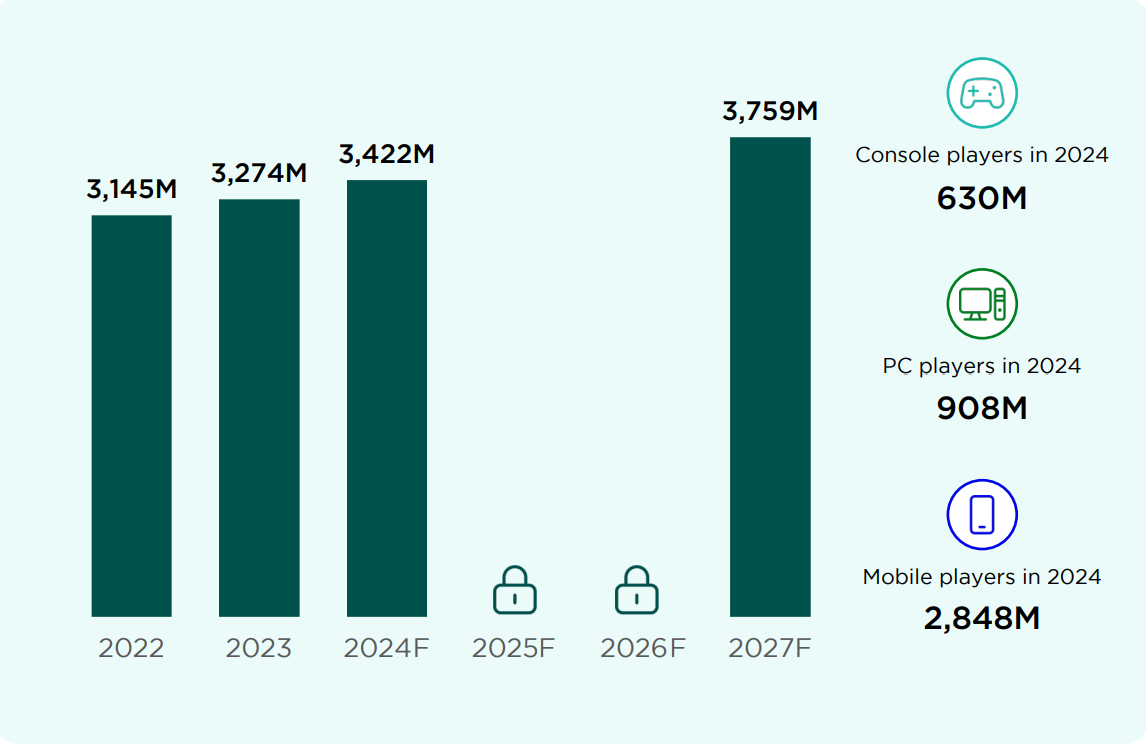
\includegraphics[width = 0.5\textwidth]{Imagenes/Newzoo_Players.png}
	\caption{Jugadores globales 2022-2024 y predicción en 2027.Newzoo}
	\label{fig:NewzooPlayers}
\end{figure}

Además en el mismo informe se comenta el porcentaje de jugadores de cada región ocupando más de la mitad, un 53\% los jugadores pacifico asiáticos como se muestra en la figura \ref{fig:NewzooPlayersReg}.
Con esos crecimientos y estos datos viene la necesidad de adaptar los videojuegos a diferentes lenguajes y culturas a través de los procesos de internacionalización ({\textit{I18N}}) y localización ({\textit{L10N}}) para poder ser publicados en otras regiones y países.
\begin{figure}[H]
	\centering
	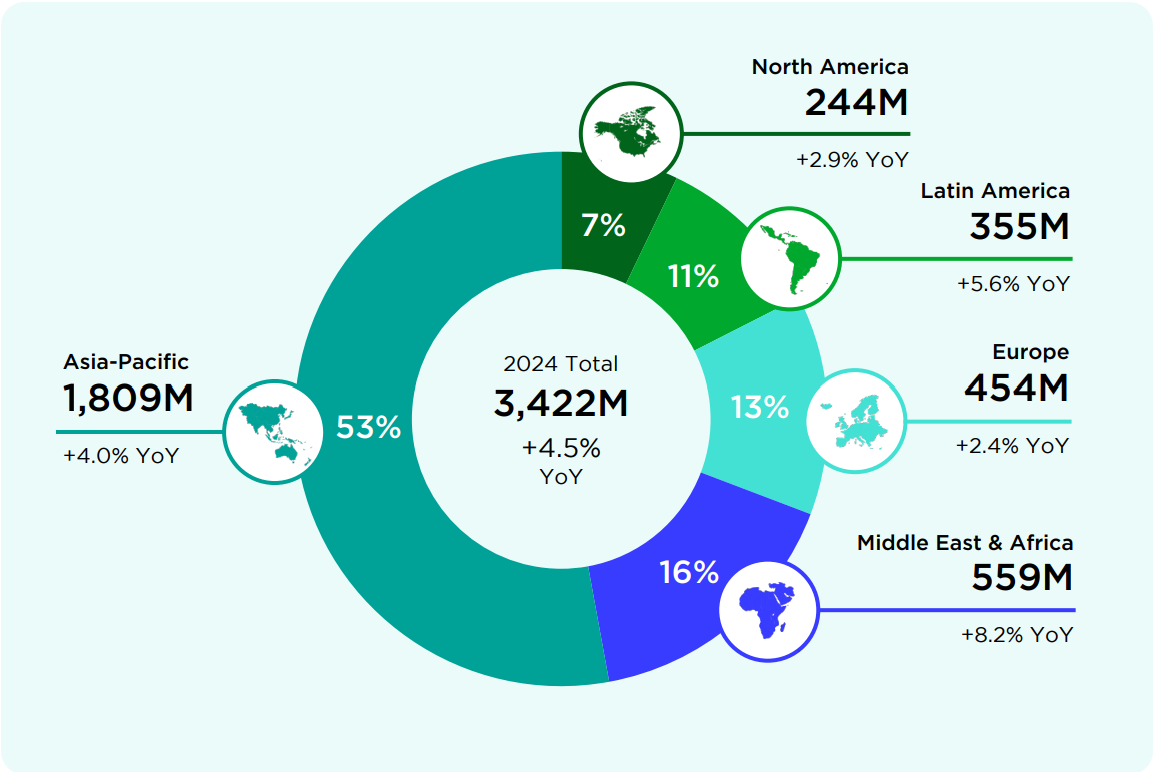
\includegraphics[width = 0.5\textwidth]{Imagenes/Newzoo_Players_Region.png}
	\caption{Porcentaje de jugadores de cada región. Newzoo}
	\label{fig:NewzooPlayersReg}
\end{figure}
La internacionalización es el proceso por el cual un videojuego se prepara desde sus etapas iniciales de desarrollo para soportar diferentes culturas e idiomas, de tal manera que no haya que realizar grandes modificaciones en el código para introducirlos.
Por otra parte, la localización es el proceso por el cual se traducen y adaptan los textos, gráficos y recursos de un videojuego para las diferentes culturas en las que éste se va a comercializar.

Durante ambos de estos procesos se pueden producir distintos tipos de errores (como errores de traducción o errores de visualización). Aquí es donde entra el \textit{Localization Quality Assurance} (o LQA). Este proceso se encarga de revisar y probar las distintas partes del videojuego para asegurarse de que no se produzca ninguno de estos errores y el producto final sea adecuado para las culturas y el público objetivo.

Hasta ahora este proceso ha sido un trabajo manual en el que los probadores comprueban meticulosamente cada texto y como éstos se visualizan dentro del videojuego, lo cual requiere de una gran cantidad de tiempo y recursos. Aunque existen herramientas para comprobar la corrección de las traducciones y los textos automáticamente, sin embargo, no se puede decir lo mismo en lo referente a comprobar que los textos se visualicen correctamente en el contexto del videojuego.

Teniendo en cuenta lo expuesto en los párrafos anteriores anterior, nuestra motivación para este trabajo es poder automatizar las pruebas sobre los procesos de internacionalización y localización, de forma que se puedan
ahorrar tiempo y recursos en estos campos y dedicarlos a otros más importantes. Para conseguir esto, vamos a utilizar técnicas de visión por computador y Reconocimiento óptico de caracteres \textit{(OCR,Optical Character Recognition)}
de forma que a partir de una captura de pantalla del videojuego, se pueda extraer el texto y realizar distintas comprobaciones y pruebas sobre él.


\section{Objetivos}
El objetivo principal en este trabajo es el diseño y la implementación de una herramienta que ayude en la automatización del QA en la localización.
Para lograr el objetivo principal, se plantea los siguientes objetivos secundarios: 
\begin{enumerate}

	\item Investigar sobre el proceso y las herramientas utilizadas en LQA, además de los errores más comunes en internacionalización y localización.
	\item Investigar sobre OCRs y cómo utilizarlas, para elegir una adecuada a nuestras especificaciones, realizando pruebas y comparaciones entre ellas.
	\item Diseñar una serie de tests automáticos basado en OCR para los posibles errores lingüísticos.
	\item Despliegue de la herramienta en una imagen de Docker para que pueda desplegarse en cualquier equipo.
	\item Integrar el OCR para usarlo como entrada de datos a los tests. Hacer mejoras para que el OCR de el máximo acierto posible.
	\item Evaluar nuestra herramienta para asegurar de que produce un porcentaje de acierto adecuado.
\end{enumerate}
\section{Plan de trabajo}
Para conseguir nuestros objetivos, seguiremos los siguientes pasos:
\begin{enumerate}
	\item Investigar y entender como funciona el proceso de internacionalización(\ref{sec:Internacionalización}), localización(\ref{sec:Localization}), el proceso de LQA(\ref{sec:LQA}) y los errores de lingüísticos más comunes(\ref{sec:Errores de localizacion}) que se producen a la hora de elaborar un videojuego. 
	\item Elegir de los errores más comunes de localización aquellas que estén relacionados con errores de caracteres o posiciones que sea posible ser detectado utilizando una OCR.(\ref{sec:Descripción de los tests})
	\item Elaborar una serie de tests que sean capaz de detectar si existe algún error de localización específico teniendo información de entrada de la OCR.(\ref{sec:Implementación de los tests})
	\item Investigar sobre distintos OCRs, ver como funcionan, como usarlos para detectar texto en imágenes, como entrenar un modelo sabiendo el idioma y la fuente usada.(\ref{sec:Seleccion de libreria de OCR})
	\item Hacer una evaluación con los OCRs seleccionados teniendo en cuenta el tiempo y el porcentaje de acierto.Buscar formas que aumente ese porcentaje de acierto.(\ref{sec:Mejoras en el reconocimiento})
	\item Hacer una evaluación por separado del funcionamiento de cada módulo (OCR, test).
	\item Unificar ambos módulos y hacer una evaluación completa de la herramienta.
	\item Generar una salida que sea fácilmente interpretado por un ser humano. 
	
\end{enumerate}
\section{Conclusion}
En conclusión, la industria de los videojuegos ha estado evolucionando de forma rápida, por lo que surge nuevas necesidades como llevar el videojuego de un idioma a otro adaptándose al país o la región. Para ello es necesario técnicas como la internacionalización y la localización en el videojuego. Para ahorrar trabajo humano, se propone un herramienta que pueda automatizar las pruebas sobre los procesos de internacionalización y localización.
